\documentclass[11pt,a4paper]{report}
\usepackage[textwidth=37em,vmargin=30mm]{geometry}
\usepackage{calc,xunicode,amsmath,amssymb,paralist,enumitem,tabu,booktabs,datetime2,xeCJK,xeCJKfntef,listings}
\usepackage{tocloft,fancyhdr,tcolorbox,xcolor,graphicx,eso-pic,xltxtra,xelatexemoji}

\newcommand{\envyear}[0]{2025}
\newcommand{\envdatestr}[0]{2025-04-28}
\newcommand{\envfinaldir}[0]{webdb/2025/20250428/final}

\usepackage[hidelinks]{hyperref}
\hypersetup{
    colorlinks=false,
    pdfpagemode=FullScreen,
    pdftitle={Web Digest - \envdatestr}
}

\setlength{\cftbeforechapskip}{10pt}
\renewcommand{\cftchapfont}{\rmfamily\bfseries\large\raggedright}
\setlength{\cftbeforesecskip}{2pt}
\renewcommand{\cftsecfont}{\sffamily\small\raggedright}

\setdefaultleftmargin{2em}{2em}{1em}{1em}{1em}{1em}

\usepackage{xeCJK,xeCJKfntef}
\xeCJKsetup{PunctStyle=plain,RubberPunctSkip=false,CJKglue=\strut\hskip 0pt plus 0.1em minus 0.05em,CJKecglue=\strut\hskip 0.22em plus 0.2em}
\XeTeXlinebreaklocale "zh"
\XeTeXlinebreakskip = 0pt


\setmainfont{Brygada 1918}
\setromanfont{Brygada 1918}
\setsansfont{IBM Plex Sans}
\setmonofont{JetBrains Mono NL}
\setCJKmainfont{Noto Serif CJK SC}
\setCJKromanfont{Noto Serif CJK SC}
\setCJKsansfont{Noto Sans CJK SC}
\setCJKmonofont{Noto Sans CJK SC}

\setlength{\parindent}{0pt}
\setlength{\parskip}{8pt}
\linespread{1.15}

\lstset{
	basicstyle=\ttfamily\footnotesize,
	numbersep=5pt,
	backgroundcolor=\color{black!5},
	showspaces=false,
	showstringspaces=false,
	showtabs=false,
	tabsize=2,
	captionpos=b,
	breaklines=true,
	breakatwhitespace=true,
	breakautoindent=true,
	linewidth=\textwidth
}






\newcommand{\coverpic}[2]{
    % argv: itemurl, authorname
    Cover photo by #2~~(\href{#1}{#1})
}
\newcommand{\makeheader}[0]{
    \begin{titlepage}
        % \newgeometry{hmargin=15mm,tmargin=21mm,bmargin=12mm}
        \begin{center}
            
            \rmfamily\scshape
            \fontspec{BaskervilleF}
            \fontspec{Old Standard}
            \fontsize{59pt}{70pt}\selectfont
            WEB\hfill DIGEST
            
            \vfill
            % \vskip 30pt
            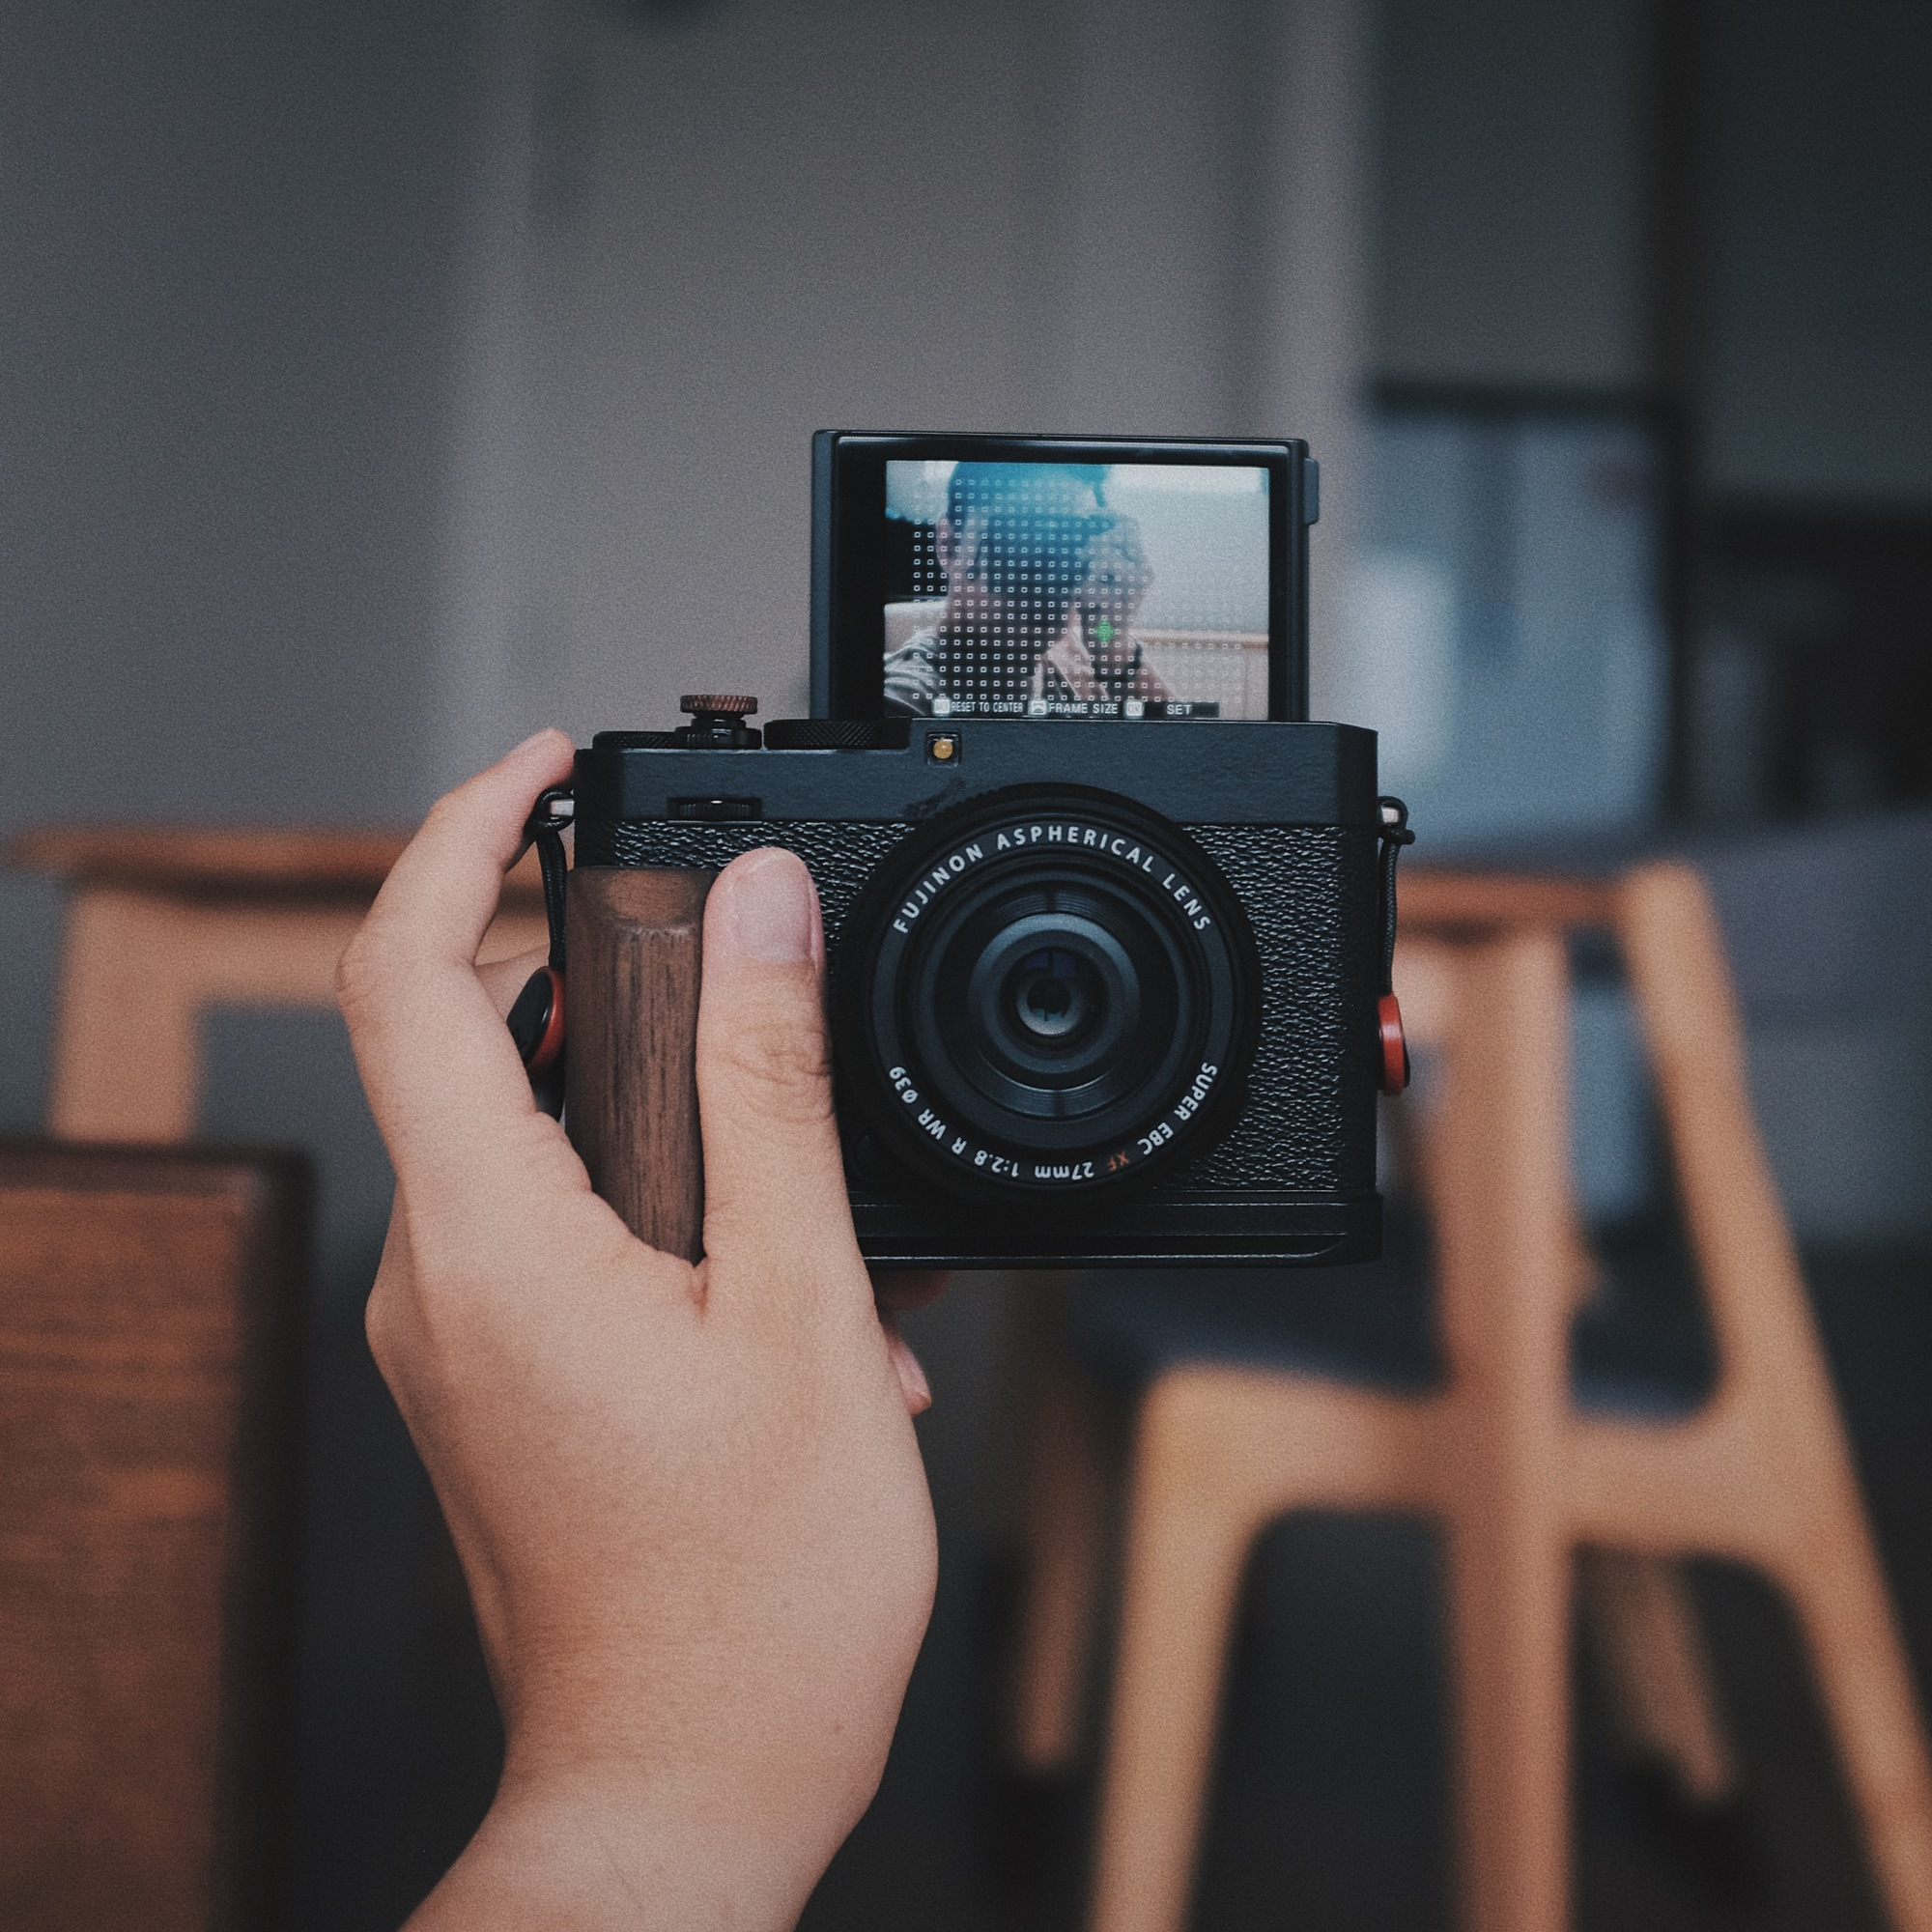
\includegraphics[width=\linewidth]{\envfinaldir/coverpic-prod.jpg}\par
            % \vskip 30pt
            \vfill

            \normalsize\rmfamily\scshape
            \copyright{} The Web Digest Project \hfill\large \envdatestr
        \end{center}
    \end{titlepage}
    % \restoregeometry
}
\newcommand{\simplehref}[1]{%
    \textcolor{blue!80!green}{\href{#1}{#1}}%
}
\renewcommand{\contentsname}{\center\Huge\sffamily\bfseries Contents\par\vskip 20pt}
\newcounter{ipartcounter}
\setcounter{ipartcounter}{0}
\newcommand{\ipart}[1]{
    % \vskip 20pt
    \clearpage
    \stepcounter{ipartcounter}
    \phantomsection
    \addcontentsline{toc}{chapter}{#1}
    % \begin{center}
    %     \Huge
    %     \sffamily\bfseries
    %     #1
    % \end{center}
    % \vskip 20pt plus 7pt
}
\newcounter{ichaptercounter}
\setcounter{ichaptercounter}{0}
\newcommand{\ichapter}[1]{
    % \vskip 20pt
    \clearpage
    \stepcounter{ichaptercounter}
    \phantomsection
    \addcontentsline{toc}{section}{\numberline{\arabic{ichaptercounter}}#1}
    \begin{center}
        \Huge
        \sffamily\bfseries
        #1
    \end{center}
    \vskip 20pt plus 7pt
}
\newcommand{\entrytitlefont}[1]{\subsection*{\raggedright\Large\sffamily\bfseries#1}}
\newcommand{\entryitemGeneric}[2]{
    % argv: title, url
    \parbox{\linewidth}{
        \entrytitlefont{#1}\par\vskip 5pt
        \footnotesize\ttfamily\mdseries
        \simplehref{#2}
    }\vskip 11pt plus 11pt minus 1pt
}
\newcommand{\entryitemGithub}[3]{
    % argv: title, url, desc
    \parbox{\linewidth}{
        \entrytitlefont{#1}\par\vskip 5pt
        \footnotesize\ttfamily\mdseries
        \simplehref{#2}\par\vskip 5pt
        \small\rmfamily\mdseries#3
    }\vskip 11pt plus 11pt minus 1pt
}
\newcommand{\entryitemAp}[3]{
    % argv: title, url, desc
    \parbox{\linewidth}{
        \entrytitlefont{#1}\par\vskip 5pt
        \footnotesize\ttfamily\mdseries
        \simplehref{#2}\par\vskip 5pt
        \small\rmfamily\mdseries#3
    }\vskip 11pt plus 11pt minus 1pt
}
\newcommand{\entryitemHackernews}[3]{
    % argv: title, hnurl, rawurl
    % \parbox{\linewidth}{
    %     \entrytitlefont{#1}\par\vskip 5pt
    %     \footnotesize\ttfamily\mdseries
    %     \simplehref{#3}\par
    %     \textcolor{black!50}{\href{#2}{#2}}
    % }\vskip 11pt plus 11pt minus 1pt
    \begin{minipage}{\linewidth}
            \entrytitlefont{#1}\par\vskip 5pt
            \footnotesize\ttfamily\mdseries
            \simplehref{#3}\par
            \textcolor{black!50}{\href{#2}{#2}}
    \end{minipage}\par\vskip 11pt plus 11pt minus 1pt
}







\begin{document}

\makeheader

\tableofcontents\clearpage




\ipart{Developers}
\ichapter{Hacker News}
\entryitemTwoLinks{Business co-founders in tech startups are less valuable than they think}{https://news.ycombinator.com/item?id=43814497}{https://verdikapuku.com/posts/business-founders-are-less-valuable-than-they-think/}

\entryitemTwoLinks{Internet in a Box}{https://news.ycombinator.com/item?id=43814433}{https://internet-in-a-box.org/}

\entryitemTwoLinks{How a single line of code could brick your iPhone}{https://news.ycombinator.com/item?id=43814360}{https://rambo.codes/posts/2025-04-24-how-a-single-line-of-code-could-brick-your-iphone}

\entryitemTwoLinks{OpenBSD 7.7 Released}{https://news.ycombinator.com/item?id=43814058}{https://www.openbsd.org/77.html}

\entryitemTwoLinks{Read the Obits}{https://news.ycombinator.com/item?id=43813175}{https://thereader.mitpress.mit.edu/the-creativity-hack-no-one-told-you-about-read-the-obits/}

\entryitemTwoLinks{Did 5G Kill the IMSI Catcher?}{https://news.ycombinator.com/item?id=43813083}{https://zetier.com/5g-imsi-catcher/}

\entryitemTwoLinks{Libogc (Wii homebrew library) discovered to contain code stolen from RTEMS}{https://news.ycombinator.com/item?id=43812995}{https://github.com/fail0verflow/hbc/blob/80a80251f83f1993c272c58e471d040f3eb1dee9/README.md}

\entryitemTwoLinks{TmuxAI: AI-Powered, Non-Intrusive Terminal Assistant}{https://news.ycombinator.com/item?id=43812646}{https://tmuxai.dev/}

\entryitemTwoLinks{We're building a dystopia just to make people click on ads [video]}{https://news.ycombinator.com/item?id=43812379}{https://www.ted.com/talks/zeynep\_tufekci\_we\_re\_building\_a\_dystopia\_just\_to\_make\_people\_click\_on\_ads}

\entryitemTwoLinks{Reverse geocoding is hard}{https://news.ycombinator.com/item?id=43812323}{https://shkspr.mobi/blog/2025/04/reverse-geocoding-is-hard/}

\entryitemTwoLinks{Wikipedia: Database Download}{https://news.ycombinator.com/item?id=43811732}{https://en.wikipedia.org/wiki/Wikipedia:Database\_download}

\entryitemTwoLinks{Shardines: SQLite3 Database-per-Tenant with ActiveRecord}{https://news.ycombinator.com/item?id=43811400}{https://blog.julik.nl/2025/04/a-can-of-shardines}

\entryitemTwoLinks{Mesmerizing Interlocking Geometric Patterns Produced with Japanese Woodworking}{https://news.ycombinator.com/item?id=43810724}{https://www.smithsonianmag.com/smithsonian-institution/see-the-mesmerizing-interlocking-geometric-patterns-produced-with-this-ancient-japanese-woodworking-technique-180986494/}

\entryitemTwoLinks{ZFS: Apple's new filesystem that wasn't (2016)}{https://news.ycombinator.com/item?id=43810566}{https://ahl.dtrace.org/2016/06/15/apple\_and\_zfs/}

\entryitemTwoLinks{U.S. autism data project sparks uproar over ethics, privacy and intent}{https://news.ycombinator.com/item?id=43810561}{https://www.washingtonpost.com/health/2025/04/25/autism-registry-privacy-rfk-research/}

\entryitemTwoLinks{Chongqing, the Largest City – In Pictures}{https://news.ycombinator.com/item?id=43809915}{https://www.theguardian.com/world/gallery/2025/apr/27/chongqing-the-worlds-largest-city-in-pictures}

\entryitemTwoLinks{Show HN: Remote-Controlled IKEA Deathstar Lamp}{https://news.ycombinator.com/item?id=43809841}{https://gitlab.com/sephalon/deathstar\_lamp}

\entryitemTwoLinks{How to program a text adventure in C}{https://news.ycombinator.com/item?id=43809638}{https://helderman.github.io/htpataic/htpataic01.html}

\entryitemTwoLinks{CSS Zen Garden}{https://news.ycombinator.com/item?id=43809484}{https://csszengarden.com/}

\entryitemTwoLinks{Open-source interactive C tutorial in the browser}{https://news.ycombinator.com/item?id=43809092}{https://www.learn-c.org/}\ichapter{Phoronix}
\entryitemGeneric{\hskip 0pt{}Linux 6.15-rc4 Released With Performance Regression Fix, Corrected Bcachefs Case Folding}{https://www.phoronix.com/news/Linux-6.15-rc4-Released}

\entryitemGeneric{\hskip 0pt{}OpenBSD 7.7 Released With AMD SEV Guest Bits, Initial Radeon RX 9070 GPU Support}{https://www.phoronix.com/news/OpenBSD-7.7-Released}

\entryitemGeneric{\hskip 0pt{}FFmpeg Merges Decoder For Samsung's APV - Advanced Professional Video Codec}{https://www.phoronix.com/news/FFmpeg-Merges-APV-Decoder}

\entryitemGeneric{\hskip 0pt{}Deferred THP Insertion Nearing The Linux Kernel To Help Avoid Memory Waste}{https://www.phoronix.com/news/Linux-TDP-Defer-Insertion-Soon}

\entryitemGeneric{\hskip 0pt{}XPG Alpha Wireless Gaming Mouse Being Quirked For Linux Support}{https://www.phoronix.com/news/XPGA-Alpha-Mouse-Linux-Support}

\entryitemGeneric{\hskip 0pt{}The Linux Kernel's SHA-256 Code Being Improved Upon For Easier \& Performant Use}{https://www.phoronix.com/news/Linux-SHA256-Crypto-Refactoring}

\entryitemGeneric{\hskip 0pt{}Mold 2.38 Linker Adds Support For LLVM's CREL Format}{https://www.phoronix.com/news/Mold-2.38-Linker}

\entryitemGeneric{\hskip 0pt{}Zblock Compressed Slab Memory Allocator Looks Like It Could Be Coming In Linux 6.16}{https://www.phoronix.com/news/Zblock-Allocator-Linux-6.16-MM}

\entryitemGeneric{\hskip 0pt{}Fair DRM Scheduler v4 Running Well On Steam Deck, "Looks Solid"}{https://www.phoronix.com/news/Fair-DRM-Scheduler-v4}\ichapter{GitHub}
\entryitemWithDescription{\hskip 0pt{}aquasecurity/trivy}{https://github.com/aquasecurity/trivy}{Find vulnerabilities, misconfigurations, secrets, SBOM in containers,
Kubernetes, code repositories, clouds and more\\
Language: Go\\
Stars: 25719\\
Forks: 2510}

\entryitemWithDescription{\hskip 0pt{}khoj-ai/khoj}{https://github.com/khoj-ai/khoj}{Your AI second brain. Self-hostable. Get answers from the web or your
docs. Build custom agents, schedule automations, do deep research. Turn
any online or local LLM into your personal, autonomous AI (gpt, claude,
gemini, llama, qwen, mistral). Get started - free.\\
Language: Python\\
Stars: 29337\\
Forks: 1637}

\entryitemWithDescription{\hskip 0pt{}tracel-ai/burn}{https://github.com/tracel-ai/burn}{Burn is a next generation Deep Learning Framework that
doesn\textquotesingle t compromise on flexibility, efficiency and
portability.\\
Language: Rust\\
Stars: 10527\\
Forks: 540}\ichapter{Dribbble}
\entryitemGeneric{\hskip 0pt{}Tallybreeze Logo Design - Accounting Automation for Property}{https://dribbble.com/shots/25946704-Tallybreeze-Logo-Design-Accounting-Automation-for-Property}

\entryitemGeneric{\hskip 0pt{}Bismuth}{https://dribbble.com/shots/25942596-Bismuth}

\entryitemGeneric{\hskip 0pt{}Quora Logo Redesign Concept}{https://dribbble.com/shots/25941918-Quora-Logo-Redesign-Concept}

\entryitemGeneric{\hskip 0pt{}Cute Viking Brand Mascot}{https://dribbble.com/shots/25943003-Cute-Viking-Brand-Mascot}

\entryitemGeneric{\hskip 0pt{}Rhino Dragon}{https://dribbble.com/shots/25945050-Rhino-Dragon}

\entryitemGeneric{\hskip 0pt{}Minimalist Z Logo Design // For Sale}{https://dribbble.com/shots/25941466-Minimalist-Z-Logo-Design-For-Sale}

\entryitemGeneric{\hskip 0pt{}Travel Startup Branding for Holidu: visual identity brand design}{https://dribbble.com/shots/25916676-Travel-Startup-Branding-for-Holidu-visual-identity-brand-design}

\entryitemGeneric{\hskip 0pt{}Betpanda}{https://dribbble.com/shots/25937317-Betpanda}

\entryitemGeneric{\hskip 0pt{}Unused Netomi Logo Concept}{https://dribbble.com/shots/25937558-Unused-Netomi-Logo-Concept}

\entryitemGeneric{\hskip 0pt{}Crypto Portfolio Tracker App}{https://dribbble.com/shots/25936470-Crypto-Portfolio-Tracker-App}

\entryitemGeneric{\hskip 0pt{}Geometric M Logo Design - Letter, Monogram}{https://dribbble.com/shots/25936398-Geometric-M-Logo-Design-Letter-Monogram}

\entryitemGeneric{\hskip 0pt{}Hand-Lettering Samples v1}{https://dribbble.com/shots/25938484-Hand-Lettering-Samples-v1}

\entryitemGeneric{\hskip 0pt{}RedBird Films}{https://dribbble.com/shots/25938378-RedBird-Films}

\entryitemGeneric{\hskip 0pt{}Colorful M - Logo Design // For SALE}{https://dribbble.com/shots/25937554-Colorful-M-Logo-Design-For-SALE}

\entryitemGeneric{\hskip 0pt{}Fundly Branding - Fintech company}{https://dribbble.com/shots/25936018-Fundly-Branding-Fintech-company}

\entryitemGeneric{\hskip 0pt{}Bismuth}{https://dribbble.com/shots/25933886-Bismuth}

\entryitemGeneric{\hskip 0pt{}boundless}{https://dribbble.com/shots/25930426-boundless}

\entryitemGeneric{\hskip 0pt{}Logo Design for Premium Online Store}{https://dribbble.com/shots/25931384-Logo-Design-for-Premium-Online-Store}

\entryitemGeneric{\hskip 0pt{}Answering Agent AI}{https://dribbble.com/shots/25932675-Answering-Agent-AI}

\entryitemGeneric{\hskip 0pt{}Visual Identity: Biometric verification layer for secure Web3}{https://dribbble.com/shots/25931676-Visual-Identity-Biometric-verification-layer-for-secure-Web3}

\entryitemGeneric{\hskip 0pt{}Tempora Logo Design - Hourglass, Time, Sand Clock}{https://dribbble.com/shots/25926528-Tempora-Logo-Design-Hourglass-Time-Sand-Clock}

\entryitemGeneric{\hskip 0pt{}Astrology Mobile App UI}{https://dribbble.com/shots/25927329-Astrology-Mobile-App-UI}

\entryitemGeneric{\hskip 0pt{}Website for a Fintech Company ✦ Kony}{https://dribbble.com/shots/25927385-Website-for-a-Fintech-Company-Kony}

\entryitemGeneric{\hskip 0pt{}OltreFluire}{https://dribbble.com/shots/25914855-OltreFluire}


\ipart{Developers~~~~(zh-Hans)}
\ichapter{Solidot}
\entryitemGeneric{\hskip 0pt{}20 个省份人口自然增长为负}{https://www.solidot.org/story?sid=81160}

\entryitemGeneric{\hskip 0pt{}4chan 恢复上线}{https://www.solidot.org/story?sid=81159}

\entryitemGeneric{\hskip 0pt{}微软向 Copilot+ PC 推送 Windows Recall 功能}{https://www.solidot.org/story?sid=81158}

\entryitemGeneric{\hskip 0pt{}美国民主党和共和党如何引用科学文献}{https://www.solidot.org/story?sid=81157}

\entryitemGeneric{\hskip 0pt{}特朗普政府瞄准维基百科}{https://www.solidot.org/story?sid=81156}

\entryitemGeneric{\hskip 0pt{}雅虎有意收购 Chrome}{https://www.solidot.org/story?sid=81155}

\entryitemGeneric{\hskip 0pt{}苹果计划将印度制造的 iPhone 出口到美国以避开关税}{https://www.solidot.org/story?sid=81154}

\entryitemGeneric{\hskip 0pt{}科学家开发出人造绿叶}{https://www.solidot.org/story?sid=81153}

\entryitemGeneric{\hskip 0pt{}VS Code 分支上的 C/C++ 扩展停止工作}{https://www.solidot.org/story?sid=81152}

\entryitemGeneric{\hskip 0pt{}社交媒体已成为过去}{https://www.solidot.org/story?sid=81151}

\entryitemGeneric{\hskip 0pt{}美国年轻男性放弃接受大学教育的人数创记录}{https://www.solidot.org/story?sid=81150}

\entryitemGeneric{\hskip 0pt{}韩监管机构称 DeepSeek 未经许可将用户信息传输到境外}{https://www.solidot.org/story?sid=81149}

\entryitemGeneric{\hskip 0pt{}新 Android 间谍软件瞄准俄罗斯前线军人}{https://www.solidot.org/story?sid=81148}

\entryitemGeneric{\hskip 0pt{}Waymo 每周提供 25 万次付费无人驾驶出租车服务}{https://www.solidot.org/story?sid=81147}

\entryitemGeneric{\hskip 0pt{}一种肉食毛虫会披着猎物残骸在蛛网上游弋}{https://www.solidot.org/story?sid=81146}

\entryitemGeneric{\hskip 0pt{}DeepMind 发布 Lyria 2 音乐生成模型}{https://www.solidot.org/story?sid=81145}

\entryitemGeneric{\hskip 0pt{}倭黑猩猩雌性通过结盟压制雄性保住权力}{https://www.solidot.org/story?sid=81144}\ichapter{V2EX}
\entryitemGeneric{\hskip 0pt{}[问与答] 你们那有交警进入封闭管理园区内部贴违停的情况}{https://www.v2ex.com/t/1128524}

\entryitemGeneric{\hskip 0pt{}[Android] 三星的手机或者平板怎么升级系统?}{https://www.v2ex.com/t/1128522}

\entryitemGeneric{\hskip 0pt{}[生活] 加密货币是否能规避掉离婚时被爆金币}{https://www.v2ex.com/t/1128521}

\entryitemGeneric{\hskip 0pt{}[问与答] M1 Pro mac 非要贴屏幕膜的话你们选什么品牌 反光少?不贴膜好多划痕、裸屏维护成本很高}{https://www.v2ex.com/t/1128520}

\entryitemGeneric{\hskip 0pt{}[酷工作] 分享近期 AI 创业搭建技术栈的一些想法,以及招聘!}{https://www.v2ex.com/t/1128519}

\entryitemGeneric{\hskip 0pt{}[分享创造] 免费职业规划神器: SWOT 分析与多款职业咨询工具,助你职场腾飞!}{https://www.v2ex.com/t/1128518}

\entryitemGeneric{\hskip 0pt{}[问与答] iPhone 可以越狱后修改销售地区?比如国行改成美版的设置 这样就没有 app 网络权限控制了}{https://www.v2ex.com/t/1128517}

\entryitemGeneric{\hskip 0pt{}[分享创造] AnyVoice.net 只需要 3 秒钟就可以复刻任何人的声音,逼真得让人难以置信}{https://www.v2ex.com/t/1128515}

\entryitemGeneric{\hskip 0pt{}[问与答] 为何外版无锁的 512G 巨魔 11 收半天收不到、难道都用国行了}{https://www.v2ex.com/t/1128513}

\entryitemGeneric{\hskip 0pt{}[程序员] 我用 Cursor 开发上架了一个 Chrome 扩展插件:将新标签页打造为 RSS 阅读器}{https://www.v2ex.com/t/1128512}

\entryitemGeneric{\hskip 0pt{}[问与答] 求推荐晚高峰速度也很快的机场}{https://www.v2ex.com/t/1128511}

\entryitemGeneric{\hskip 0pt{}[问与答] 4K 预算安卓机求推荐}{https://www.v2ex.com/t/1128510}

\entryitemGeneric{\hskip 0pt{}[问与答] 大模型的出现,会进一步蚕食论坛平台的市场吗?}{https://www.v2ex.com/t/1128509}

\entryitemGeneric{\hskip 0pt{}[问与答] 要疯了, pyinstall 打包的 exe,打开总是报错 ModuleNotFoundError: No module named 'jieba'}{https://www.v2ex.com/t/1128508}

\entryitemGeneric{\hskip 0pt{}[宽带症候群] 梯子推荐,支持国外的 ipv6}{https://www.v2ex.com/t/1128507}

\entryitemGeneric{\hskip 0pt{}[程序员] 发现个新语言 c3-lang, 朋友位怎么看}{https://www.v2ex.com/t/1128506}

\entryitemGeneric{\hskip 0pt{}[梦] 爱情、回忆、死亡与真实感}{https://www.v2ex.com/t/1128505}

\entryitemGeneric{\hskip 0pt{}[路由器] USB 供电是否稳定?}{https://www.v2ex.com/t/1128504}

\entryitemGeneric{\hskip 0pt{}[VXNA] 申请收录个人博客: Macin}{https://www.v2ex.com/t/1128503}

\entryitemGeneric{\hskip 0pt{}[VPS] 出 iepl 三网转发}{https://www.v2ex.com/t/1128502}

\entryitemGeneric{\hskip 0pt{}[分享发现] 就事论事, JD 外卖这黑稿有点夸张了吧?}{https://www.v2ex.com/t/1128501}

\entryitemGeneric{\hskip 0pt{}[摄影] 意大利 多洛米蒂}{https://www.v2ex.com/t/1128500}

\entryitemGeneric{\hskip 0pt{}[问与答] 如何快捷地调试 appletv 的网络}{https://www.v2ex.com/t/1128497}

\entryitemGeneric{\hskip 0pt{}[宽带症候群] 使用公网 IPV6 的 DDNS 方案,用不了 RDP}{https://www.v2ex.com/t/1128495}

\entryitemGeneric{\hskip 0pt{}[分享发现] 吐槽淘宝平台售后}{https://www.v2ex.com/t/1128493}

\entryitemGeneric{\hskip 0pt{}[问与答] 买个了研华工控机主板 AIMB-782QG2,安装 i7-3770 无法启动}{https://www.v2ex.com/t/1128492}

\entryitemGeneric{\hskip 0pt{}[奇思妙想] 轻量云好像都搭建不了域控,无论阿里还是腾讯。只能用 ECS/CVM}{https://www.v2ex.com/t/1128491}

\entryitemGeneric{\hskip 0pt{}[中文] 为什么喜欢用「新」字}{https://www.v2ex.com/t/1128490}

\entryitemGeneric{\hskip 0pt{}[问与答] 关于 Augment+idea 无法自动应用代码}{https://www.v2ex.com/t/1128485}

\entryitemGeneric{\hskip 0pt{}[Android] 一加 13t 值得入手吗}{https://www.v2ex.com/t/1128484}

\entryitemGeneric{\hskip 0pt{}[宽带症候群] 墙又高了,还有什么可靠的爬墙方法?}{https://www.v2ex.com/t/1128483}

\entryitemGeneric{\hskip 0pt{}[Apple] Chrome for macOS 滚动条滚动的感觉能调到像 Safari 一样利落吗?}{https://www.v2ex.com/t/1128482}

\entryitemGeneric{\hskip 0pt{}[macOS] macOS 部分应用窗口的标题栏,有条线在闪烁,忽黑忽白}{https://www.v2ex.com/t/1128480}

\entryitemGeneric{\hskip 0pt{}[Python] 关于 Python 学习问题}{https://www.v2ex.com/t/1128477}

\entryitemGeneric{\hskip 0pt{}[Apple] iPhone 14PM ios 16 刷 ipcc 64 或者 63 刷进去重启掉的进来}{https://www.v2ex.com/t/1128476}

\entryitemGeneric{\hskip 0pt{}[Apple] Perplexity iOS/MacOS 客户端登陆报错解决}{https://www.v2ex.com/t/1128475}

\entryitemGeneric{\hskip 0pt{}[OpenAI] 怎么感觉 ChatGPT 最近变得很有"血肉"感}{https://www.v2ex.com/t/1128473}

\entryitemGeneric{\hskip 0pt{}[问与答] 我的 chrome 浏览器,右边滚动条有时候出现,但经常消失看不到,大家知道是什么原因么}{https://www.v2ex.com/t/1128472}

\entryitemGeneric{\hskip 0pt{}[NAS] [求助]笔记本电脑上传到 NAS 只有百兆速度}{https://www.v2ex.com/t/1128471}

\entryitemGeneric{\hskip 0pt{}[NAS] 大家有啥办法解决 NAS+3.5 寸盘+风扇 噪音很大的问题?}{https://www.v2ex.com/t/1128469}

\entryitemGeneric{\hskip 0pt{}[Planet] what is this ?}{https://www.v2ex.com/t/1128468}

\entryitemGeneric{\hskip 0pt{}[程序员] Stash macOS 可以在请求列表页面设置规则吗?}{https://www.v2ex.com/t/1128467}

\entryitemGeneric{\hskip 0pt{}[职场话题] 三年前端经验 offer 选择, 京东 or 携程,友友们给点建议}{https://www.v2ex.com/t/1128466}

\entryitemGeneric{\hskip 0pt{}[程序员] 前端是否有办法根据用户设备性能自动减弱过渡动画效果?}{https://www.v2ex.com/t/1128465}

\entryitemGeneric{\hskip 0pt{}[旅行] 求 Osprey 小鹰背包推荐}{https://www.v2ex.com/t/1128463}

\entryitemGeneric{\hskip 0pt{}[软件] 一年了, WPS 鼠标显示位置与鼠标选中位置不符的问题还没解决}{https://www.v2ex.com/t/1128462}

\entryitemGeneric{\hskip 0pt{}[信息安全] 前端 npm 包如果长期不更新,是否不会带来除了 XSS 以外的安全风险? Angular 相关的东西整天搞 Breaking Changes,向下兼容性极差,根本没法更新}{https://www.v2ex.com/t/1128461}

\entryitemGeneric{\hskip 0pt{}[问与答] 关于眼镜,镜架的选择大家有什么建议吗?}{https://www.v2ex.com/t/1128460}

\entryitemGeneric{\hskip 0pt{}[问与答] 自考本是否应该考研?}{https://www.v2ex.com/t/1128459}

\entryitemGeneric{\hskip 0pt{}[iPhone] iPhone 不下载菜鸟可以收集所有取件码吗?}{https://www.v2ex.com/t/1128458}


\ipart{Generic News}
\ichapter{联合早报}
\entryitemWithDescription{黎康:魔都的B面}{https://www.zaobao.com/news/china/story20250426-6241474}{``确实这几年上海的城市公共建设很好,但你有没有去看过一些老旧小区的环境?小区里电线横飞,绿化基本毫无规划;进入楼道,你会感觉回到20年前\ldots\ldots'' 上一篇``早点------沪上闲语''发表后,收到一封读者来信。这位上海市民告诉我,在装点城市门面的郁金香背后,如果走进上海的老旧小区,会看到这座城市的另一面……}

\entryitemWithDescription{新闻人间:从``不懂球的胖子''到改革推手——刘国梁}{https://www.zaobao.com/news/china/story20250426-6238850}{中国乒乓球协会星期三(4月23日)突然宣布,刘国梁主动辞去主席一职。这一消息迅速引发体坛热议,有球迷为他的离开感到惋惜,也有体育评论员开始审视他在任期内的功与过。 刘国梁自2018年起担任乒协主席,如今在第二任期尚未结束之际中途请辞,外界难免有诸多猜测。星期三当天,他以主席身份在乒协会议上作最后一次发言时,几度哽咽,甚至当场落泪。 他在记者会上透露,早在去年巴黎奥运会结束后,便已向上级表达了去意……}

\entryitemWithDescription{中国据报考虑暂停加征部分美国产品125\%关税}{https://www.zaobao.com/news/china/story20250425-6245926}{中国政府据报考虑暂停对部分美国进口产品加征125\%的关税,受访学者认为此举主要考虑中国企业的生存需要,与中美是否开启贸易谈判无关。 据彭博社引述知情人士报道,中国政府正考虑取消对美国的医疗设备,以及乙烷等工业化学品加征的报复性关税。中国是全球最大的塑料制造国,但部分工厂依赖从美国进口的乙烷。中国医院也需要美国生产的磁共振成像和超声仪器等医疗设备。 知情人士称,飞机租赁也可能豁免关税……}

\entryitemWithDescription{中国美国商会白皮书:五分之一美企不再视中国为优先投资地}{https://www.zaobao.com/news/china/story20250425-6245113}{中国美国商会的调查显示,五分之一的在华美国企业不再将中国列为优先的投资目的地。 该商会星期五(4月25日)发布由100余名中国美国商会会员企业代表共同撰写的2025年《美国企业在中国白皮书》。 白皮书指出,中美两国关系日益紧张,已连续五年成为在华美资企业面临的首要商业挑战,超过了合规风险和来自中国企业的竞争压力……}

\entryitemWithDescription{中国发布生态调查报告 称菲律宾捕捞现场发现人为弃置物}{https://www.zaobao.com/news/china/story20250425-6244616}{(北京讯)中国多家自然生态机构星期五(4月25日)联合公布一份调查报告,评估铁线礁、牛轭礁珊瑚礁的生态系统状况,称菲律宾所谓``中国在铁线礁倾倒珊瑚碎屑等言论''毫无科学和事实依据。 中国自然资源部微信公号分别发表了这份题为《铁线礁、牛轭礁珊瑚礁生态系统调查报告》的中英文版本,参与编制的机构包括中国自然资源部南海发展研究院、南海生态中心等……}

\entryitemWithDescription{香港公共场所明年起设更多禁烟区 违例罚款提高一倍}{https://www.zaobao.com/news/china/story20250425-6245064}{为了进一步降低吸烟率,香港特区政府将由明年起在更多公共场所设立禁烟区,并把违例吸烟的罚款金额提高一倍至3000港元(508新元)。 相关条例草案星期五(4月25日)刊宪,列明从明年元旦起,禁止在等候公共交通工具、等候进入电影院、医院、公众游乐场地、体育场等地方的划定范围吸烟。违者罚款由1500港元倍增至3000港元……}

\entryitemWithDescription{两韩国顶尖半导体专家 退休后被中国高校任用}{https://www.zaobao.com/news/china/story20250425-6244895}{(首尔讯)中国正通过从海外引进顶尖人才,与美国争夺高科技主导权。韩国两名``国宝级''顶尖专家退休后在本国受到冷落,未能找到合适研究职位,目前已被中国高等学府任用。 据韩国《中央日报》报道,韩国知名碳纳米管专家李永熙去年11月正式受聘于湖北工业大学半导体与量子研究所……}

\entryitemWithDescription{美国传降对陆关税又强化对台论述 分析:谈判或拿台湾当筹码}{https://www.zaobao.com/news/china/story20250425-6244227}{华盛顿释出降低对华关税信号、寻求谈判之际,美国星期三(4月23日)首次在联合国安理会批评北京误用联大2758号决议;更在同一天派遣军舰穿越台湾海峡。受访学者分析,这些作为现阶段暂与关税战没有直接关联,但不排除美国总统特朗普接下来可能利用台湾问题作为对华谈判筹码。 特朗普本周透露考虑大幅度降低对华关税,希望与中国达成``公平的协议'',同时又声称美国每天都同中国直接联系……}

\entryitemWithDescription{韩咏红:特朗普关税从``解放日''走到``妥协日''了?}{https://www.zaobao.com/news/china/story20250425-6240846}{美国总统特朗普在4月2日宣布对等关税政策,短短20天后,特朗普的高姿态已难以为继。特朗普在4月9日就已调整过一次战术,暂缓对其他国家课征对等关税,集中火力单挑中国;而今,特朗普恐怕又要眨眼了,对中国商品课征的145\%关税也可能显著下调。 特朗普近日罕见地对中国伸出橄榄枝,表示考虑大幅度降低对华关税,显露出急于与中国达成协议。但中国偏是表现得不着急……}

\entryitemWithDescription{学者:中国以2+2机制拉拢东南亚国家抗衡美国}{https://www.zaobao.com/news/china/story20250424-6240690}{受访学者分析,在中美关系因贸易战而全面恶化的大背景下,中国正以``外交、国防2+2对话机制''为新抓手,积极拉拢亚细安成员国,以抗衡美国在本区域的影响力,预计中国接下来将推动与更多区域国家建立2+2机制。 中国和印度尼西亚星期一(4月21日)在北京举行外长、防长对话机制下的首次部长级会议,两国在2023年就建立2+2对话机制。中国官方称,这是中国在全球建立的首个部长级2+2机制……}

\entryitemWithDescription{中埃空军首次联训 学者:中国初步具备向中东快速战略投送能力}{https://www.zaobao.com/news/china/story20250424-6240357}{中国空军上周派出多架战斗机、预警机、运输机与空中加油机前往埃及,进行两军首次联训。这是中国空军首次以完整作战体系进行跨洲机动。 受访学者认为,这是中国空军现代化进程的里程碑,有助于发展长途奔袭的技战术;这也标志着中国初步具备向中东进行快速战略投送的能力。 据中国国防部消息,中国与埃及两国空军于4月中旬至5月上旬,在埃及空军基地组织代号为``文明之鹰-2025''的联合训练……}

\entryitemWithDescription{台湾收紧民众申领大陆证照规定 持大陆定居证也将被撤销台湾身份}{https://www.zaobao.com/news/china/story20250424-6239789}{(台北综合讯)台湾再度收紧民众申领中国大陆证照的规定,持有大陆定居证的台湾民众也触犯相关法令,将丧失台湾身份。 综合《旺报》与《联合报》报道,台湾行政院公报显示,陆委会近日对《两岸条例》当中规定发布解释函令称,为确保两岸人员单一身份制度,两岸条例规定台湾人民不得在大陆地区``设有户籍'',或领用大陆地区护照,否则将丧失台湾身份……}

\entryitemWithDescription{神舟二十号成功发射 航天员将开展中国首次涡虫空间再生实验}{https://www.zaobao.com/news/china/story20250424-6239950}{(北京综合讯)中国星期四(4月24日)成功发射神舟二十号载人飞船。三名航天员将在空间站驻留约六个月,并开展中国首次涡虫空间再生实验。 综合新华社、央视新闻和《中国青年报》报道,搭载神舟二十号的长征二号F遥二十运载火箭,星期四下午5时17分在甘肃酒泉卫星发射中心点火发射。约10分钟后,神舟二十号与火箭成功分离,进入预定轨道……}

\entryitemWithDescription{台大罢免升温 朝野对抗加剧}{https://www.zaobao.com/news/china/story20250424-6240062}{台湾两大在野党将携手举办大型造势活动,抗议政府利用司法整肃异己,进行大罢免。兼任民进党主席的总统赖清德则公开肯定公民团体罢免在野党立委的行动影片,检调也持续搜索在野国民党宜兰县党部,朝野对抗情势正逐步升温……}

\entryitemWithDescription{美国国会罕见动用传唤权 调查中国三电信巨头}{https://www.zaobao.com/news/china/story20250424-6239456}{(纽约路透电)美国众议院中国问题特别委员会星期三(4月23日)罕见地动用传唤权,调查中国三大电信公司涉嫌支持中国军方和政府的行为。 据路透社报道,中国移动、中国电信和中国联通三家中国电信巨头收到该委员会的传唤通知,须回答他们是否可通过在美开展的云服务和互联网业务获取美国数据的问题。 美国两党议员持续对被指由中国主导的网络攻击事件表示担忧……}

\entryitemWithDescription{浙江一小学门外发生汽车冲撞人群事件}{https://www.zaobao.com/news/china/story20250424-6238514}{(香港综合讯)中国再发生校园伤人事件,浙江金华一所小学门外星期二(4月22日)放学时有汽车冲撞人群,伤亡人数不明。官方在事发两日后仍未发布通报,中国社媒上的相关信息均被删除。 综合《明报》《南华早报》和网媒``香港01''报道,这起事件发生在金华市苏孟乡中心小学门口,时间是星期二傍晚5时45分左右,正值放学时间。附近商户披露,有多名学生被撞……}

\entryitemWithDescription{学者:关税战伤敌一千自损八百 中美终将找到共处之道}{https://www.zaobao.com/news/china/story20250424-6238821}{美国总统特朗普祭出对等关税将届满一个月,如今传出可能降低对华关税,定居美国的资深华人学者赵全胜指出,中美领导阶层有一批人长期相信对方马上要垮台,但关税战让双方意识到,这无疑是``伤敌一千,自损八百'',因此迟早会找到共处之道。 特朗普4月2日宣布全面实施对等关税,随后在9日紧急暂缓90天,让各国争取与美国谈判的时间与空间,唯独对中国不断加码;北京也不甘示弱,提出相应反制……}

\entryitemWithDescription{打击电诈犯罪扩至纵深地带 缅甸向中国移交920余名嫌犯}{https://www.zaobao.com/news/china/story20250424-6238307}{(北京综合讯)中国与缅甸加大打击电信网络诈骗犯罪合作力度,两国最近一个月的合作执法行动,已从缅北地区扩大到当阳、勐休等缅甸纵深地带。 中国公安部官网星期三(4月23日)通报,缅甸执法部门近日将在当地抓获的920余名中国籍涉诈犯罪嫌疑人,通过云南西双版纳打洛口岸全部移交中国警方。 通报称,缅北电诈犯罪集团遭受重创,但部分涉诈人员为逃避打击,向当阳、勐休等纵深地带转移藏匿,继续实施跨境电诈……}

\entryitemWithDescription{沈泽玮:魔幻山城的中国式现代化演绎}{https://www.zaobao.com/news/china/story20250424-6234868}{时隔12年因工作再访重庆,春夏交替之际迎来烈日当空,与当年冬季旅游行走于山城迷雾的印象截然不同。 5000架无人机灯光秀,既展现科技力量也打造视觉盛宴;科企创始人讲述营商环境不断优化;村委会主任手捧涪陵榨菜分享东方酱腌菜``走出去''成果;火车司机传递通关速度如何带动互联互通跨境贸易;公安局交巡警总队科研处综合科科长讲述数字化赋能超大城市治理;社区党委书记分享中国特色``民主村''的前身今世……}

\entryitemWithDescription{中国网购平台将全面取消``仅退款''}{https://www.zaobao.com/news/china/story20250423-6234242}{在中国官方整治``内卷式竞争''的背景下,中国电商平台将全面取消``仅退款''选项。受访学者认为,此举有助行业回归良性竞争,是对电商市场的一次纠偏。 据《北京商报》报道,拼多多、淘宝、抖音、快手、京东等多个中国电商平台,星期二(4月22日)修改有关``仅退款''的相关条款,消费者申请``退款不退货'',将由商家自主处理……}

\entryitemWithDescription{3月人民币跨境收付占比刷新历史纪录}{https://www.zaobao.com/news/china/story20250423-6233857}{(华盛顿彭博电)随着美元的全球吸引力减弱、中美贸易紧张局势上升,3月中国投资者和贸易公司在国际结算中对人民币的使用大幅增加,创下历史纪录。 彭博社基于中国国家外汇管理局星期二(4月22日)公布的数据计算,3月中国大陆境内个人和机构的跨境业务中,人民币使用占比达 54.3\%,总额7249亿美元(9502亿新元)……}






\clearpage
\leavevmode\vfill
\footnotesize

Copyright \copyright{} 2023-2025 Neruthes and other contributors.

This document is published with CC BY-NC-ND 4.0 license.

The entries listed in this newsletter may be copyrighted by their respective creators.

This newsletter is generated by the Web Digest project.

The newsletters are also delivered via Telegram channel \CJKunderline{\href{https://t.me/webdigestchannel}{https://t.me/webdigestchannel}}.\\
RSS feed is available at \CJKunderline{\href{https://webdigest.pages.dev/rss.xml}{https://webdigest.pages.dev/rss.xml}}.

This newsletter is available in PDF at
\CJKunderline{\href{https://webdigest.pages.dev/}{https://webdigest.pages.dev/}}.

The source code being used to generate this newsletter is available at\\
\CJKunderline{\href{https://github.com/neruthes/webdigest}{https://github.com/neruthes/webdigest}}.

This newsletter is also available in
\CJKunderline{\href{http://webdigest.pages.dev/readhtml/\envyear/WebDigest-20250428.html}{HTML}} and
\CJKunderline{\href{https://github.com/neruthes/webdigest/blob/master/markdown/\envyear/WebDigest-20250428.md}{Markdown}}.


\coverpic{https://unsplash.com/photos/woman-poses-with-neon-lights-in-red-silhouette-\_zfYXxFPFOY}{Jay Soundo}


\end{document}
